\section{搜索问题}
\label{sec:rs-problem}

只能评价候选时，搜索到底在面对什么？先把目标、允许的候选和一次评价的回报固定下来，再看局部改善为什么会停滞。

\paragraph{目标、候选和一次评价}
全章考虑的问题写成
\begin{equation}
 \min_{\bm{x}\in\bm{C}}f(\bm{x}),
 \label{eq:rs-problem}
\end{equation}
其中$\bm{C}$是允许的候选集合，$f$是待最小化的代价，$f^\star$和$\bm{x}^\star$是最优值和最优解。$\bm{C}$可以是$\mathbb{R}^n$的一块区域，也可以是有限集合，比如所有长度为$n$的0--1串，或者$n$个元素的所有排列。

算法与问题之间只有一种接触方式：提交一个候选$\bm{x}$，收到一个数。这叫一次\term{评价}（evaluation）。收到的数不告诉我们$f$在别处的取值，也不带梯度或曲率。全章把预算记作$B$，表示允许的评价总次数；字母$T$留给后面的温度。

\paragraph{局部改善为什么会停}
看一个最小的例子。状态集合是$\{1,2,\ldots,7\}$，每个状态只与左右相邻的状态相连，代价是
\begin{equation}
 \bigl(f(1),f(2),\ldots,f(7)\bigr)=(3,\,1,\,3,\,5,\,2,\,0,\,2).
 \label{eq:rs-double-valley}
\end{equation}
全局最小在$x=6$，代价为$0$；$x=2$是另一个低谷，代价为$1$。两个低谷之间隔着代价为$5$的$x=4$。

规则“只走向更低的邻居”从$x=3$出发，下一步到$x=2$。在$x=2$，两个邻居的代价都是$3$，都比当前高，于是永远停在这里。从$1,2,3$出发都停在$x=2$，从$4,5,6,7$出发才能到达$x=6$。七个状态里有三个起点拿不到最优解，而算法在$x=2$上收不到任何“还有更好的地方”的信号。这就是图~\ref{fig:rs-two-landscapes}(a)。

连续变量也一样。考虑二维的Rastrigin函数
\begin{equation}
 f(\bm{x})=20+\sum_{i=1}^{2}\bigl(x_i^2-10\cos(2\pi x_i)\bigr).
 \label{eq:rs-rastrigin}
\end{equation}
全局最小在原点，$f^\star=0$。余弦项在每个整数点附近挖出一个小坑，在$[-5.12,5.12]^2$内共有$11^2=121$个局部极小点。

图~\ref{fig:rs-two-landscapes}(b)从四个起点运行梯度下降，每条路径都很快落进离起点最近的小坑。例如从$(-2.3,2.6)$出发，终点约为$(-1.99,2.98)$，那里的代价约为$12.9$。梯度下降在那里做的是对的事情，梯度也确实趋于零，只是这个驻点离全局最小还很远。

\begin{BookInlineFigure}
 \centering
 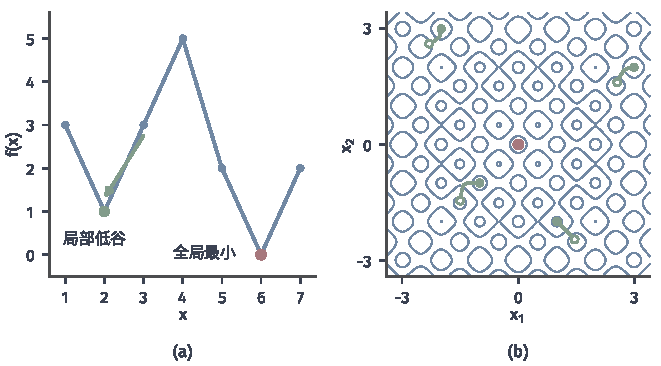
\includegraphics[width=112mm]{figures/05-optimization/05-stochastic-optimization/matplotlib/rs-two-landscapes/figure.pdf}
 \caption{两个多谷的代价。(a)七状态双谷代价~\eqref{eq:rs-double-valley}，绿色箭头是从$x=3$出发的下降，绿点是停止处，红点是全局最小。(b)二维Rastrigin函数~\eqref{eq:rs-rastrigin}的等高线（$f=8,24,40$），绿色曲线是从四个空心起点运行的梯度下降，它们都停在邻近的局部极小点（绿色实心点），红点是全局最小点。}
 \label{fig:rs-two-landscapes}
\end{BookInlineFigure}

要越过这样的障碍，算法必须做一些眼前并不划算的事：接受更差的候选，或者同时在多个地方试探。本章各方法的差别就在这里。

\paragraph{三个不同的数}
讨论算法时要分清三个数，它们经常被混为一谈。第一个是\textbf{真实目标值}$f(\bm{x})$，这是问题真正关心的量。

第二个是\textbf{读数}。评价可能含有噪声，这时收到的是
\begin{equation}
 \tilde f(\bm{x})=f(\bm{x})+\varepsilon,
 \label{eq:rs-reading}
\end{equation}
其中$\varepsilon$是这一次评价的误差。无噪声时$\tilde f=f$。第~\ref{sec:rs-noise}节之前都设无噪声。

第三个是\textbf{历史最好记录}。算法运行到第$t$次评价时，把已见的可行候选中读数最低的那个单独存下来：
\begin{equation}
 \begin{gathered}
 \bm{x}_{\mathrm{best}}^{(t)}\in\argmin\bigl\{\tilde f(\bm{x}^{(s)}):s\leq t,\ \bm{x}^{(s)}\in\bm{C}\bigr\},\\
 f_{\mathrm{best}}^{(t)}=\min_{s\leq t,\,\bm{x}^{(s)}\in\bm{C}}\tilde f(\bm{x}^{(s)}).
 \end{gathered}
 \label{eq:rs-best-record}
\end{equation}
无噪声时$f_{\mathrm{best}}^{(t)}$是真实值，而且随$t$不增。有噪声时它只是“最幸运的读数”，第~\ref{sec:rs-noise}节专门讨论这个差别。

\subsection{搜索空间}
\label{sec:rs-space}

同一个问题有不同的方式描述“从这个候选能走到哪里”。这一小节的问题是：候选的表示和移动方式怎样决定了搜索能到达什么地方？

\paragraph{三种候选，三种移动}
连续参数$\bm{x}\in\mathbb{R}^n$上最常用的移动是扰动$\bm{x}+\sigma\bm{z}$，其中$\bm{z}$是随机向量，$\sigma>0$控制尺度。一步可以到达的候选充满$\bm{x}$周围的一片区域。

二进制串$\bm{b}\in\{0,1\}^n$上的基本移动是翻位：改变一位。长度为$n$的串恰有$n$个翻位邻居，任何两个串之间相差几位，就至少需要几次翻位。

排列是把$n$个元素排成一列，$n!$种排法对应$n!$个候选。基本移动是交换两个位置上的元素。图~\ref{fig:rs-moves}把三种移动画在一起。

\begin{BookInlineFigure}
 \centering
 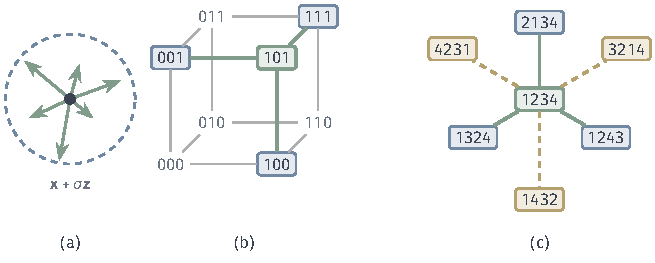
\includegraphics[width=111mm]{figures/05-optimization/05-stochastic-optimization/tikz/rs-moves/figure.pdf}
 \caption{三种候选上的移动，绿色表示当前候选及其一步移动。(a)连续参数的扰动，虚线圆表示尺度$\sigma$的量级。(b)三位二进制串构成立方体，蓝框是$101$的三个翻位邻居。(c)排列$1234$的邻居，蓝框是相邻交换，黄框和虚线是不相邻位置的交换。}
 \label{fig:rs-moves}
\end{BookInlineFigure}

把“一步能到达的候选”记为\term{邻域}（neighborhood）$\bm{N}(\bm{x})\subset\bm{C}$。邻域决定了一张图：候选是顶点，$\bm{y}\in\bm{N}(\bm{x})$就连一条边。局部低谷、爬坡路径都是相对这张图而言的，换一个邻域，低谷可能就不存在了。

\paragraph{编码要保留原问题的含义}
候选的表示必须让移动后的结果仍然有意义。例如选择问题用0--1串，第$i$位表示第$i$件物品选或不选，翻一位正是“多拿或少拿一件”，含义清楚。

把一个$0$到$15$的整数写成四位二进制，翻最高位会使整数变化$8$，翻最低位只变化$1$。从$7=0111$到相邻的$8=1000$要同时翻四位，数值上的近邻在编码上反而很远。这种表示下，翻位邻域与“数值接近”不是一回事，邻域的设计要先问清楚这一点。

\paragraph{相邻交换与任意交换}
用同一个问题比较两种邻域。平面上五个城市$A(1,4)$、$B(2,4)$、$C(3,5)$、$D(2,5)$、$E(5,0)$，距离取坐标差绝对值之和，一个访问顺序的代价是相邻两城距离之和，不返回起点。当前顺序$ABECD$的代价是
\[
 1+7+7+1=16.
\]
这条路线在中途绕向远处的$E$，然后折返，见图~\ref{fig:rs-swap-tour}(a)。

相邻交换只调换相邻的两个位置，$ABECD$的四个邻居的代价是
\[
 BAECD:17,\qquad AEBCD:18,\qquad ABCED:18,\qquad ABEDC:17.
\]
都比$16$高，所以$ABECD$是相邻交换下的局部低谷。

任意交换允许调换任何两个位置。交换$E$和$D$得到$ABDCE$，代价是
\[
 1+1+1+7=10,
\]
一步就到了五城问题的最优解，见图~\ref{fig:rs-swap-tour}(b)。

相邻交换也能到达最优解，只是要先爬坡：$ABECD\to ABCED\to ABCDE\to ABDCE$，代价依次是
\[
 16\ \to\ 18\ \to\ 12\ \to\ 10.
\]
这条路要先翻过高度为$2$的坎。同一对候选，在一种邻域下一步可达，在另一种邻域下隔着障碍。

\begin{BookInlineFigure}
 \centering
 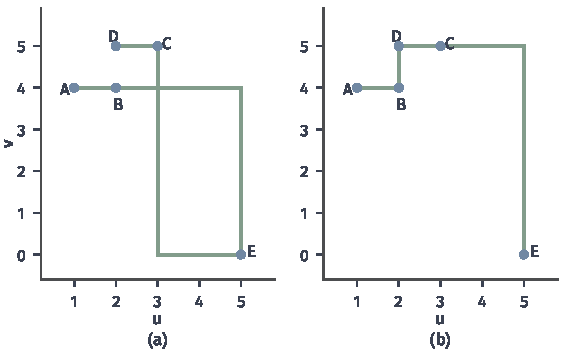
\includegraphics[width=96mm]{figures/05-optimization/05-stochastic-optimization/matplotlib/rs-swap-tour/figure.pdf}
 \caption{五城访问顺序，绿线按坐标差绝对值之和的路线画出，$u,v$是城市的横纵坐标。(a)顺序$ABECD$，长度$16$，四种相邻交换都使长度变大。(b)交换不相邻的$E$和$D$得到$ABDCE$，长度$10$。}
 \label{fig:rs-swap-tour}
\end{BookInlineFigure}

邻域并不是越大越好。五个位置时，相邻交换的邻居有$4$个，任意交换的有$10$个。任意两个排列之间，相邻交换至多需要$10$步，任意交换至多需要$4$步。

表~\ref{tab:rs-swap-neighborhood}列出这个比较。邻域大，一步能跳得远，图的直径小；代价是随机抽一个邻居时，抽到好邻居的机会被稀释，要穷举全部邻居时评价次数也更多。邻域的大小和移动尺度是算法设计中要专门决定的量，它与后面的接受规则彼此独立。

\begin{BookInlineTable}
 \centering
 \caption{$n$个元素的排列上两种交换邻域的比较，括号内是$n=5$的值。}
 \label{tab:rs-swap-neighborhood}
 \begin{tabular}{lll}
  \toprule
  & 相邻交换 & 任意交换 \\
  \midrule
  邻居个数 & $n-1$（$4$） & $n(n-1)/2$（$10$） \\
  任两排列间的最多步数 & $n(n-1)/2$（$10$） & $n-1$（$4$） \\
  是否能到达所有排列 & 能 & 能 \\
  一次移动改变的位置关系 & 小 & 可能很大 \\
  \bottomrule
 \end{tabular}
\end{BookInlineTable}

\subsection{搜索状态}
\label{sec:rs-state}

邻域回答“能走到哪里”。接下来的问题是：两次评价之间，算法手里究竟保存着什么？后面四类方法在这一点上差别最大，先把它们放在一起对比。

\paragraph{四种需要区分的对象}
\textbf{当前候选}是算法下一步移动的出发点，模拟退火就只维护这一个点。\textbf{群体成员}是同时维护的多个候选，遗传算法和粒子群属于这一类，粒子还各自带着速度。

\textbf{搜索分布参数}不是候选，而是描述“下一批候选从哪里抽”的量，例如高斯分布的中心和协方差。中心$\bm{m}$本身可能从未被评价过。\textbf{历史最好记录}是式~\eqref{eq:rs-best-record}定义的结果，它只被写入，不参与移动，除非某种算法特意使用它。

图~\ref{fig:rs-carriers}画出前三种状态，空心圆是各自的历史最好记录。表~\ref{tab:rs-state}比较它们带着什么信息。

\begin{BookInlineFigure}
 \centering
 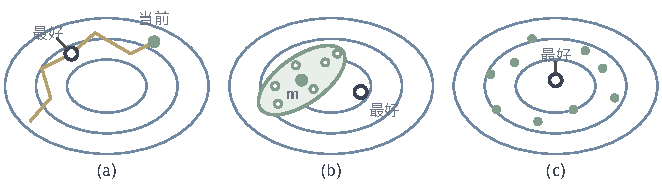
\includegraphics[width=112mm]{figures/05-optimization/05-stochastic-optimization/tikz/rs-carriers/figure.pdf}
 \caption{三种搜索状态，蓝线是目标等高线，空心圆是单独保存的历史最好记录。(a)单个当前候选（绿点）及其走过的路径（黄线），当前点可以比历史最好差。(b)搜索分布，绿点是中心$\bm{m}$，椭圆是分布的形状，空心小圆是抽到的后代，最好记录可能在椭圆外。(c)候选群体。}
 \label{fig:rs-carriers}
\end{BookInlineFigure}

\begin{BookInlineTable}
 \centering
 \caption{搜索状态承载的信息。}
 \label{tab:rs-state}
 \begin{tabular}{lll}
  \toprule
  状态 & 记住什么 & 下一批候选从哪里来 \\
  \midrule
  单个候选 & 一个点 & 这个点的邻域 \\
  搜索分布 & 中心、尺度、形状 & 从分布抽样 \\
  候选群体 & 多个点及其评价 & 成员的组合与变动 \\
  \bottomrule
 \end{tabular}
\end{BookInlineTable}

\paragraph{为什么要单独保存最好记录}
后面会看到，模拟退火有时接受更差的候选，整代替换的算法会把上一代全部丢弃。当前状态的代价因此可以上升，算法停止时手里的当前点可能比中途见过的某个点差很多。

保存记录的代价只是多存一个点。它不影响搜索的走向，却保证无噪声时交出的结果不差于任何已见的可行候选。所以无论采用什么算法，完整流程都要写上这一步。

\paragraph{与函数值方向估计的分工}
第~\ref{chap:zeroth-order-optimization}章也只用函数值：在当前点附近做差分或随机方向试探，组成梯度的估计$\hat{\bm{g}}^{(t)}$，再走一步：
\[
 \bm{x}^{(t+1)}=\bm{x}^{(t)}-\alpha^{(t)}\hat{\bm{g}}^{(t)}.
\]
它的主要对象是一个点和一个方向，分析用的是局部光滑性。

本章的主要对象是候选和选择，通常只用比较结果，也不要求$f$有导数，排列、开关这样的离散候选上根本谈不上方向。两者也有重合之处：后面第~\ref{sec:rs-es}节的高斯搜索分布，其均值的更新量可以看成平滑目标的梯度估计，这样的方法同时属于两种视角。
